\documentclass[11pt]{article} 
\usepackage{calc}
\usepackage[margin={1in,1in}]{geometry} 
\usepackage[hwkhandout]{hwk}
\usepackage[pdftitle={Calc 1
  Notes},colorlinks=true,urlcolor=blue]{hyperref}
\usepackage{tikz}

\renewcommand{\theclass}{\textsc{math}1300: calculus I}
\renewcommand{\theauthor}{Tyson Gern}
\renewcommand{\theassignment}{Optimiztion}
\renewcommand{\dateinfo}{section 4.4}

\newcommand{\ds}{\displaystyle}

\begin{document}
\drawtitle

\begin{enumerate}

\item A rectangular stock pen is to be built using a total of 600 ft
  of fencing. Part of this fencing will be used to build a fence
  across the middle of the rectangle. Find the length and width of the
  rectangle that give the maximum total area.

  \vfill

\item A rectangular box with a square base and no top is to be made of
  a total of $120\rm{cm}^2$ of cardboard.  Find the dimensions of the
  box of maximum volume.
  
  \vfill

\item Suppose that you are making a 355mL (355 cm$^3$) cyllindrical
  soda can.  The material for the top and bottom costs \$$0.002$ per
  cm$^2$ and the material for the sides costs \$$0.001$ per
  cm$^2$. What are the dimensions of the can that minimize the cost,
  and what is the minimum cost?

  \vfill

\item Find the coordinates of the point on the graph $y=\sqrt{x-2}$
  that is closest to the origin? (\textit{Hint: Minimize the square of
    the distance---this avoids square roots.})

  \vfill

\item On the same side of a long distance power cable lie two towns.
  The towns want to build a power station along the cable and use this
  to connect each town to the cable.  Where should the station be
  built in order to minimize the amount of cable used?
  \begin{center}
    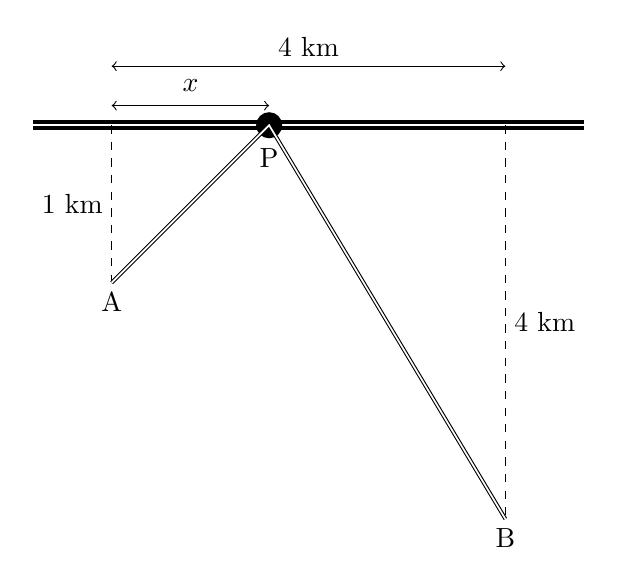
\begin{tikzpicture}[scale=1]
      \draw[<->] (1,5.75) -- (6,5.75);
      \draw[<->] (1,5.25) -- (3,5.25);
      \draw[double, ultra thick](0,5)--(7,5);
      \draw[dashed] (1,5) -- (1,3) node[below] {A};
      \draw[dashed] (6,5) -- (6,0) node[below] {B};
      \node at (.5, 4) {1 km};
      \node at (6.5, 2.5) {4 km};
      \node at (2, 5.5) {$x$};
      \node at (3.5, 6) {4 km};
      \node[circle, fill=black, label=below:P] at (3,5) {};
      \draw[double] (1,3) -- (3,5) -- (6,0);
    \end{tikzpicture}

    \textit{Ask for a hint before you start this problem!}
  \end{center}

  \vfill

\item A rectangle is inscribed in the region enclosed by the curve
  $y=9-x^2$ and the $x$-axis.  Find the dimensions of the rectangle
  with the largest area.

\end{enumerate}

\end{document}
